\section{Experiments}
\label{sec:experiments}
\subsection{Data and Evaluation Setup}
We use CRC and TIGER tissue data. Training and development follow spatial-block splits, with full $4\times$ input-footprint separation for support--query pairs and across splits. Patient and slide provenance is retained.

The remote development queue uses $300$ CRC support patches and $3{,}200$ distinct query patches from $75$ query slides. It covers the 11 tissues in Table~\ref{tab:wsi_tissue}; background contributes valid negative pixels. Among $11{,}000$ tasks, $7{,}334$ contain the target and $3{,}666$ do not. Each task has three positive and two negative support clicks, simulated from support annotations by fixed rules and shared across methods. This remote queue supports method comparison and selection. Whole-slide evaluation uses 15 slides and 152 tissue tasks. The patient cases used for whole-slide testing are absent from both the training and development sets.

\subsection{Comparisons and Metrics}
\label{sec:baselines}
We compare FewClick with SANSA, SAM, SAM2, WSI-SAM, and SAM-Med2D. Each receives the same $9{,}500$ additional target-training tasks, $2{,}375$ updates, and support clicks; evaluation uses final weights. Public pretraining, model architecture, input views, and adapted modules follow each method's configuration. The matched quantity is the additional target-data adaptation budget.

SANSA adapts its public Universal adapter for support-to-query propagation. SAM-family models use support-conditioned bridges to generate automatic dense prompts; WSI-SAM also uses fixed-rule sparse prompts. Image encoders are frozen. SANSA uses a single fine view; SAM, SAM2, and SAM-Med2D use three aligned views, and WSI-SAM uses fine and $2\times$ views. FewClick and SANSA train 7.03M and 26.33M parameters, respectively. Full initialization and adaptation configurations are provided in the supplement.

We report class-macro Dice for target-present queries and false-positive area (FPA) for target-absent queries. Small and large targets occupy $<20\%$ and $\geq20\%$ of valid query area, respectively. Precision, recall, and boundary F1 at a physical tolerance of $2\,\mu$m characterize coverage and contour quality. For WSIs, we compute Dice per slide--target pair on unique valid pixels, average across slides within each tissue, and then average the 11 tissues equally. Full-slide and strict-remote domains follow Sec.~\ref{sec:wsi}.

\subsection{Same-Slide Remote Patch Segmentation}
\begin{table}[t]
\centering
\caption{Same-slide remote segmentation on 11,000 tasks, with three positive and two negative support clicks and no query clicks. All metrics are percentages; bold marks the best value.}
\label{tab:remote}
\small
\setlength{\tabcolsep}{4pt}
\begin{tabular}{@{}lrrr@{}}
\toprule
Method & Dice $\uparrow$ & Large $\uparrow$ & FPA $\downarrow$ \\
\midrule
SAM & 30.31 & 64.40 & 27.01 \\
SAM2 & 33.60 & 66.50 & 18.91 \\
WSI-SAM & 23.81 & 50.02 & 23.43 \\
SAM-Med2D & 24.28 & 54.80 & 39.87 \\
SANSA & 41.54 & 77.22 & 14.79 \\
FewClick & \textbf{42.11} & \textbf{78.49} & \textbf{7.75} \\
\bottomrule
\end{tabular}
\end{table}

Table~\ref{tab:remote} compares the six methods on identical tasks. FewClick achieves 42.11\% target-present macro Dice, 78.49\% large-target Dice, and 7.75\% target-absent FPA. SANSA obtains 41.54\%, 77.22\%, and 14.79\%, respectively. FewClick improves the two Dice measures by 0.57 and 1.27 percentage points and reduces FPA by 7.04 points, a 47.6\% relative reduction.

Across 4,000 paired resamples of the 75 query slides, the 95\% interval is $[-8.37,-5.70]$ points for FPA and $[-0.11,1.31]$ for present Dice. The FPA interval stays below zero; the Dice interval includes zero.

\subsection{Whole-Slide Segmentation}
\begin{table}[t]
\centering
\caption{Whole-slide class-macro Dice (\%) on 15 slides and 152 tissue tasks. Each slide--target pair uses one support patch with three positive and two negative clicks. Strict remote excludes support-overlapping input footprints.}
\label{tab:wsi}
\small
\setlength{\tabcolsep}{4pt}
\begin{tabular}{@{}lrr@{}}
\toprule
Method & Full slide $\uparrow$ & Strict remote $\uparrow$ \\
\midrule
SAM & 18.86 & 16.63 \\
SAM2 & 23.58 & 21.01 \\
WSI-SAM & 15.85 & 14.25 \\
SAM-Med2D & 13.59 & 11.97 \\
SANSA & 33.23 & 30.12 \\
FewClick & \textbf{43.75} & \textbf{40.98} \\
\bottomrule
\end{tabular}
\end{table}

\begin{table*}[t]
\centering
\caption{Full-slide Dice (\%) by tissue for all six methods on the same 15 WSIs. Each tissue score averages valid slide--target pairs; $n$ is the number of contributing slides. Macro average weights the 11 tissues equally. Bold marks the highest Dice in each row.}
\label{tab:wsi_tissue}
\small
\setlength{\tabcolsep}{0.5pt}
\begin{tabularx}{\textwidth}{@{}p{0.20\textwidth}*{7}{>{\centering\arraybackslash}X}@{}}
\toprule
Tissue & $n$ & SAM & SAM2 & WSI-SAM & SAM-Med2D & SANSA & FewClick \\
\midrule
Tumor epithelium & 15 & 50.02 & 58.79 & 35.53 & 36.87 & 78.97 & \textbf{79.17} \\
Tumor stroma & 15 & 31.53 & 36.39 & 27.11 & 22.86 & 42.97 & \textbf{55.23} \\
Necrosis & 15 & 15.09 & 20.29 & 14.83 & 11.72 & 32.91 & \textbf{44.10} \\
Normal glands & 15 & 18.35 & 24.27 & 17.41 & 8.77 & 26.10 & \textbf{43.23} \\
Normal stroma & 15 & 5.68 & 9.01 & 5.61 & 5.48 & 20.80 & \textbf{25.12} \\
Submucosa/serosa & 15 & 22.75 & 25.18 & 19.94 & 19.47 & 36.15 & \textbf{49.83} \\
Muscle & 15 & 31.82 & 37.27 & 29.46 & 23.50 & 51.27 & \textbf{61.32} \\
Lymphoid aggregates & 7 & 2.17 & 2.61 & 1.51 & 1.96 & 5.46 & \textbf{34.24} \\
Mucus & 15 & 3.82 & 6.92 & 3.79 & 3.05 & 9.23 & \textbf{18.76} \\
Adipose & 15 & 22.96 & 30.58 & 16.14 & 13.59 & \textbf{49.51} & 48.67 \\
Blood & 10 & 3.22 & 8.10 & 3.01 & 2.25 & 12.13 & \textbf{21.59} \\
\midrule Macro average & -- & 18.86 & 23.58 & 15.85 & 13.59 & 33.23 & \textbf{43.75} \\
\bottomrule
\end{tabularx}
\end{table*}

\begin{figure*}[t]
\centering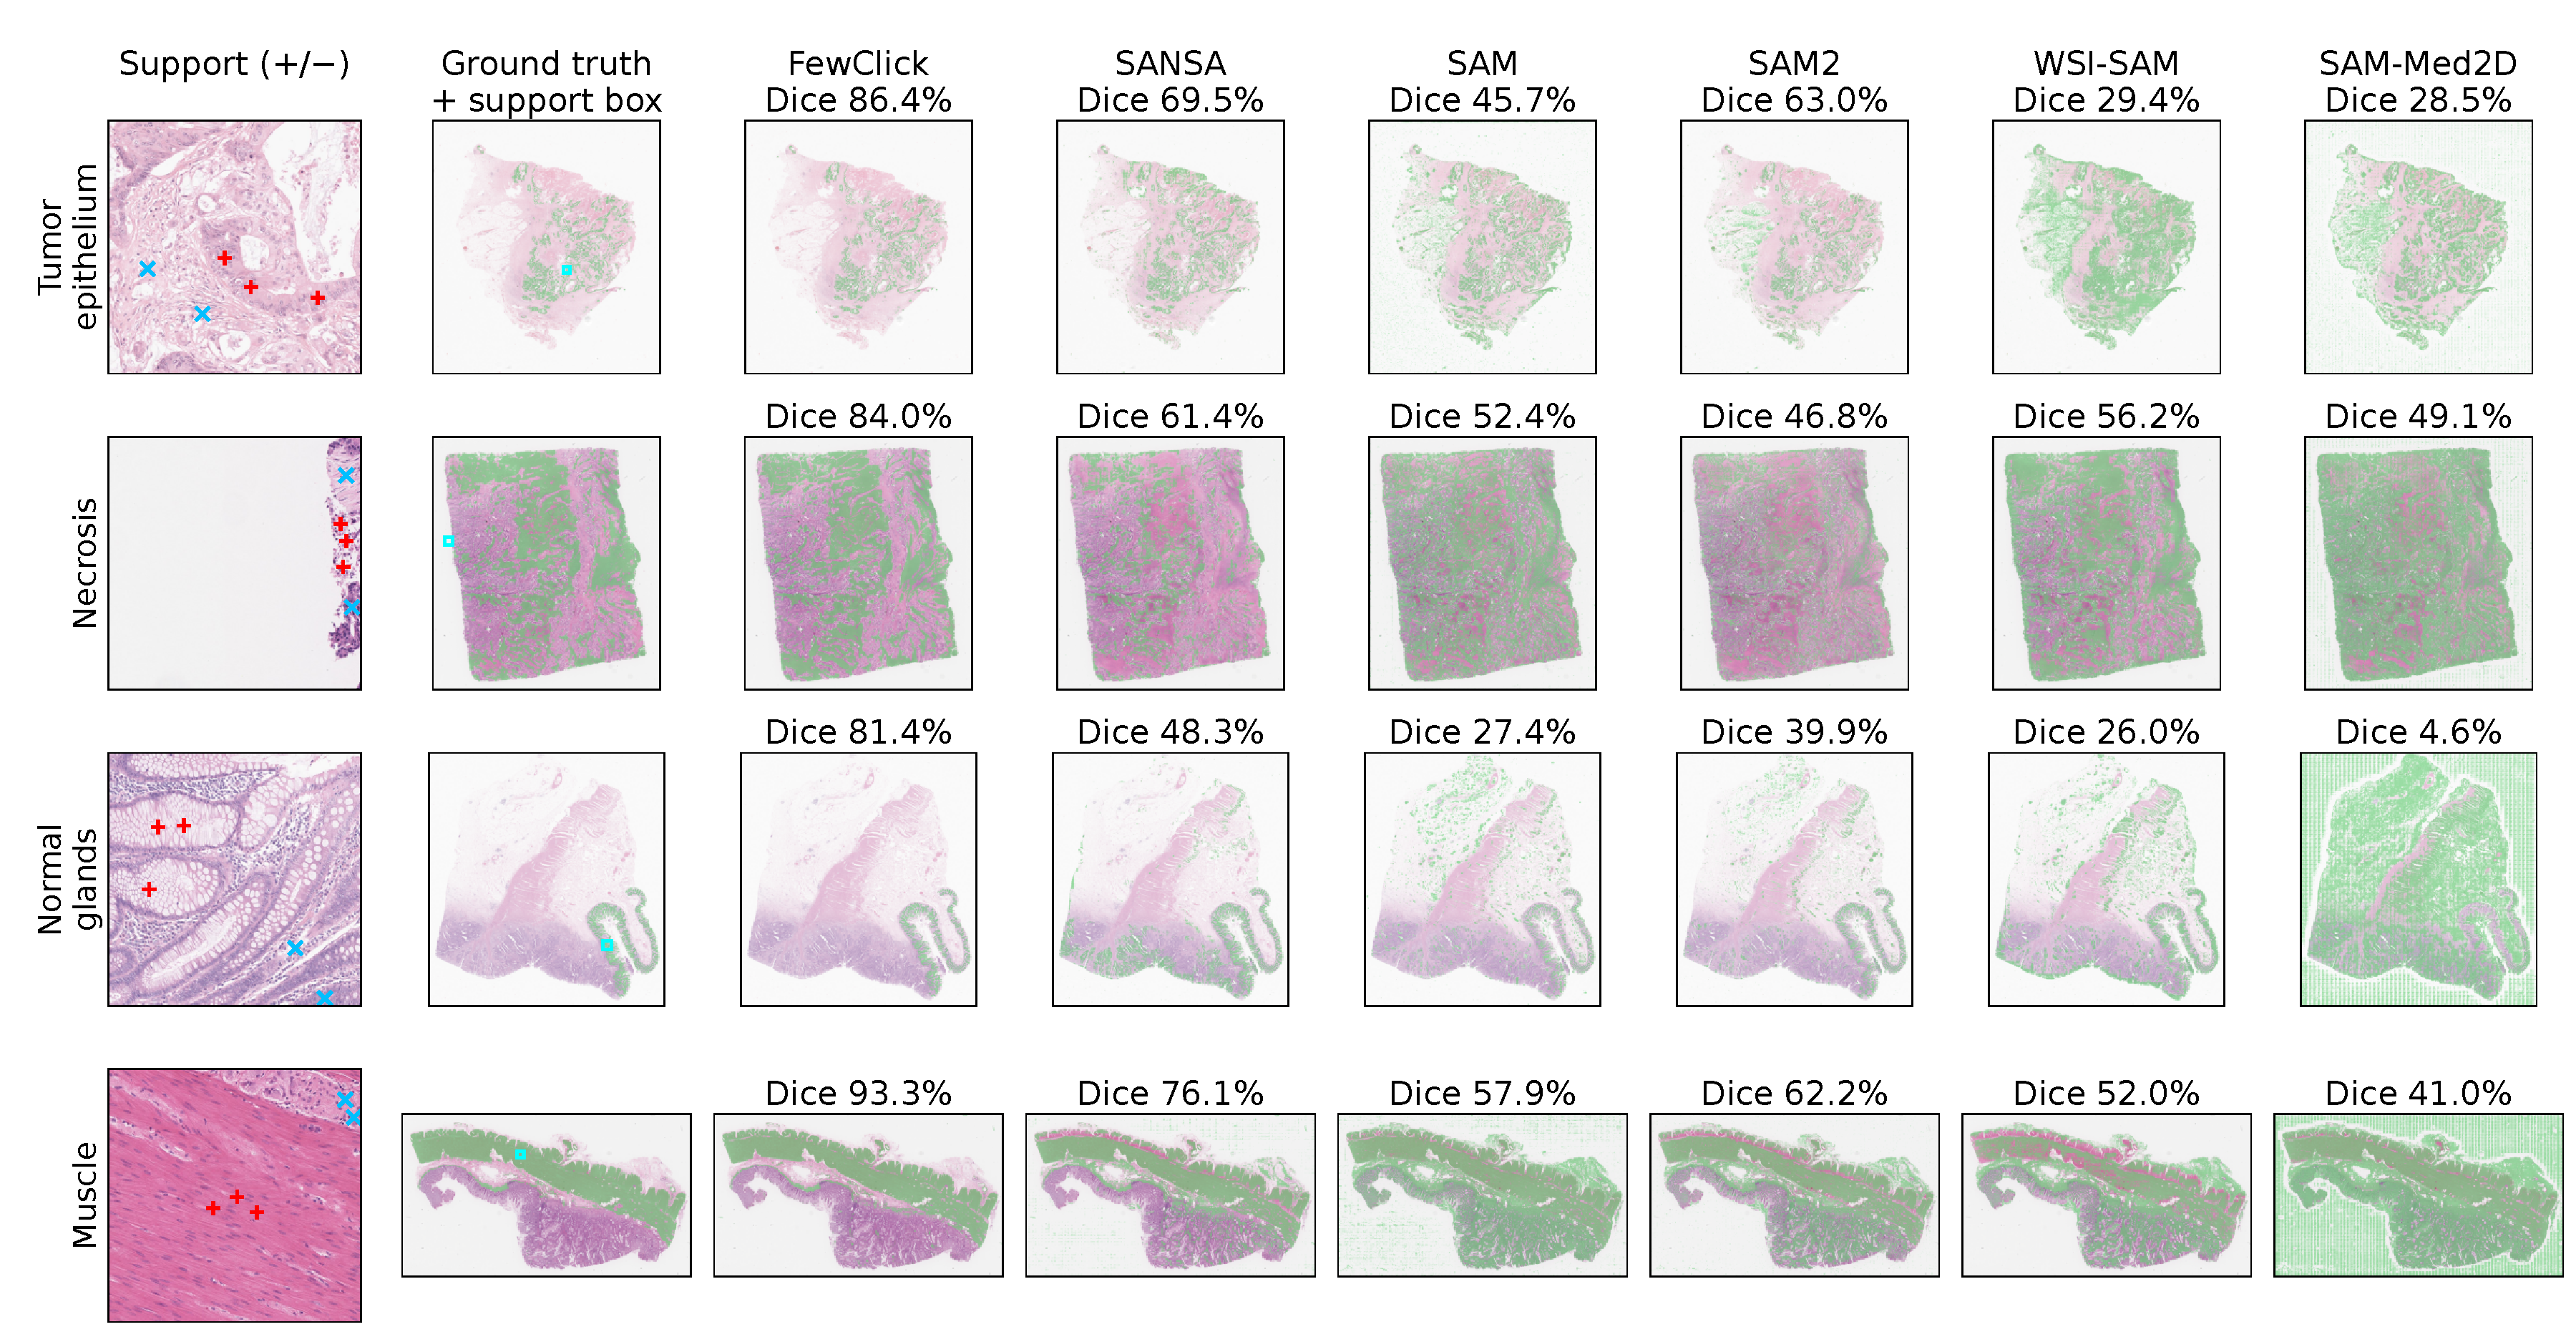
\includegraphics[width=\textwidth]{figures/figure2.pdf}
\caption{Selected whole-slide segmentation examples, each using one support set. Rows show tumor epithelium, necrosis, normal glands, and muscle; columns show support clicks, ground truth with the support box, and six-method predictions. Red plus and sky-blue cross markers denote positive and negative clicks. Green overlays denote target tissue; cyan boxes locate support patches. Panel scores are full-slide Dice for the corresponding slide--target pair, computed on full-resolution valid pixels.}
\label{fig:wsi}
\end{figure*}
The six methods complete 912 tissue--method evaluations on 15 WSIs. FewClick reaches 43.75\% full-slide macro Dice and 40.98\% strict-remote macro Dice, improving over SANSA's 33.23\% and 30.12\% by 10.52 and 10.86 points (Table~\ref{tab:wsi}). The gain persists after excluding outputs associated with support-overlapping input footprints. Averaging available tissues within each slide, FewClick outperforms SANSA on 14 of 15 slides in both domains. Paired slide-clustered bootstrap gives 95\% confidence intervals of $[7.62,13.56]$ and $[8.02,13.87]$ points for the full-slide and strict-remote gains.

FewClick improves full-slide Dice over SANSA on 10 of 11 tissues; adipose is slightly lower. Normal glands and lymphoid aggregates gain 17.13 and 28.78 points, respectively (Table~\ref{tab:wsi_tissue}). Their strict-remote gains remain 18.04 and 29.11 points, supporting transfer beyond the support neighborhood. Figure~\ref{fig:wsi} shows selected tissue examples.

\paragraph{From windows to whole slides.}
On the  formal WSIs, present-window Dice is 37.79\% for FewClick and 37.37\% for SANSA; fused whole-slide Dice is 45.65/34.85\%. Assigning each pixel to the covering window with the nearest center gives 46.41/34.70\% without overlap averaging. The whole-slide gain therefore persists before averaging. Present-window Dice averages only windows containing the target, whereas whole-slide Dice counts each valid pixel once and includes false positives in target-absent windows. In these windows, FewClick/SANSA FPA is 3.26/8.31\%. Lower absent-window FPA contributes to the larger whole-slide gain, which reflects both target coverage and rejection of non-target regions.

\begin{figure*}[t]
\centering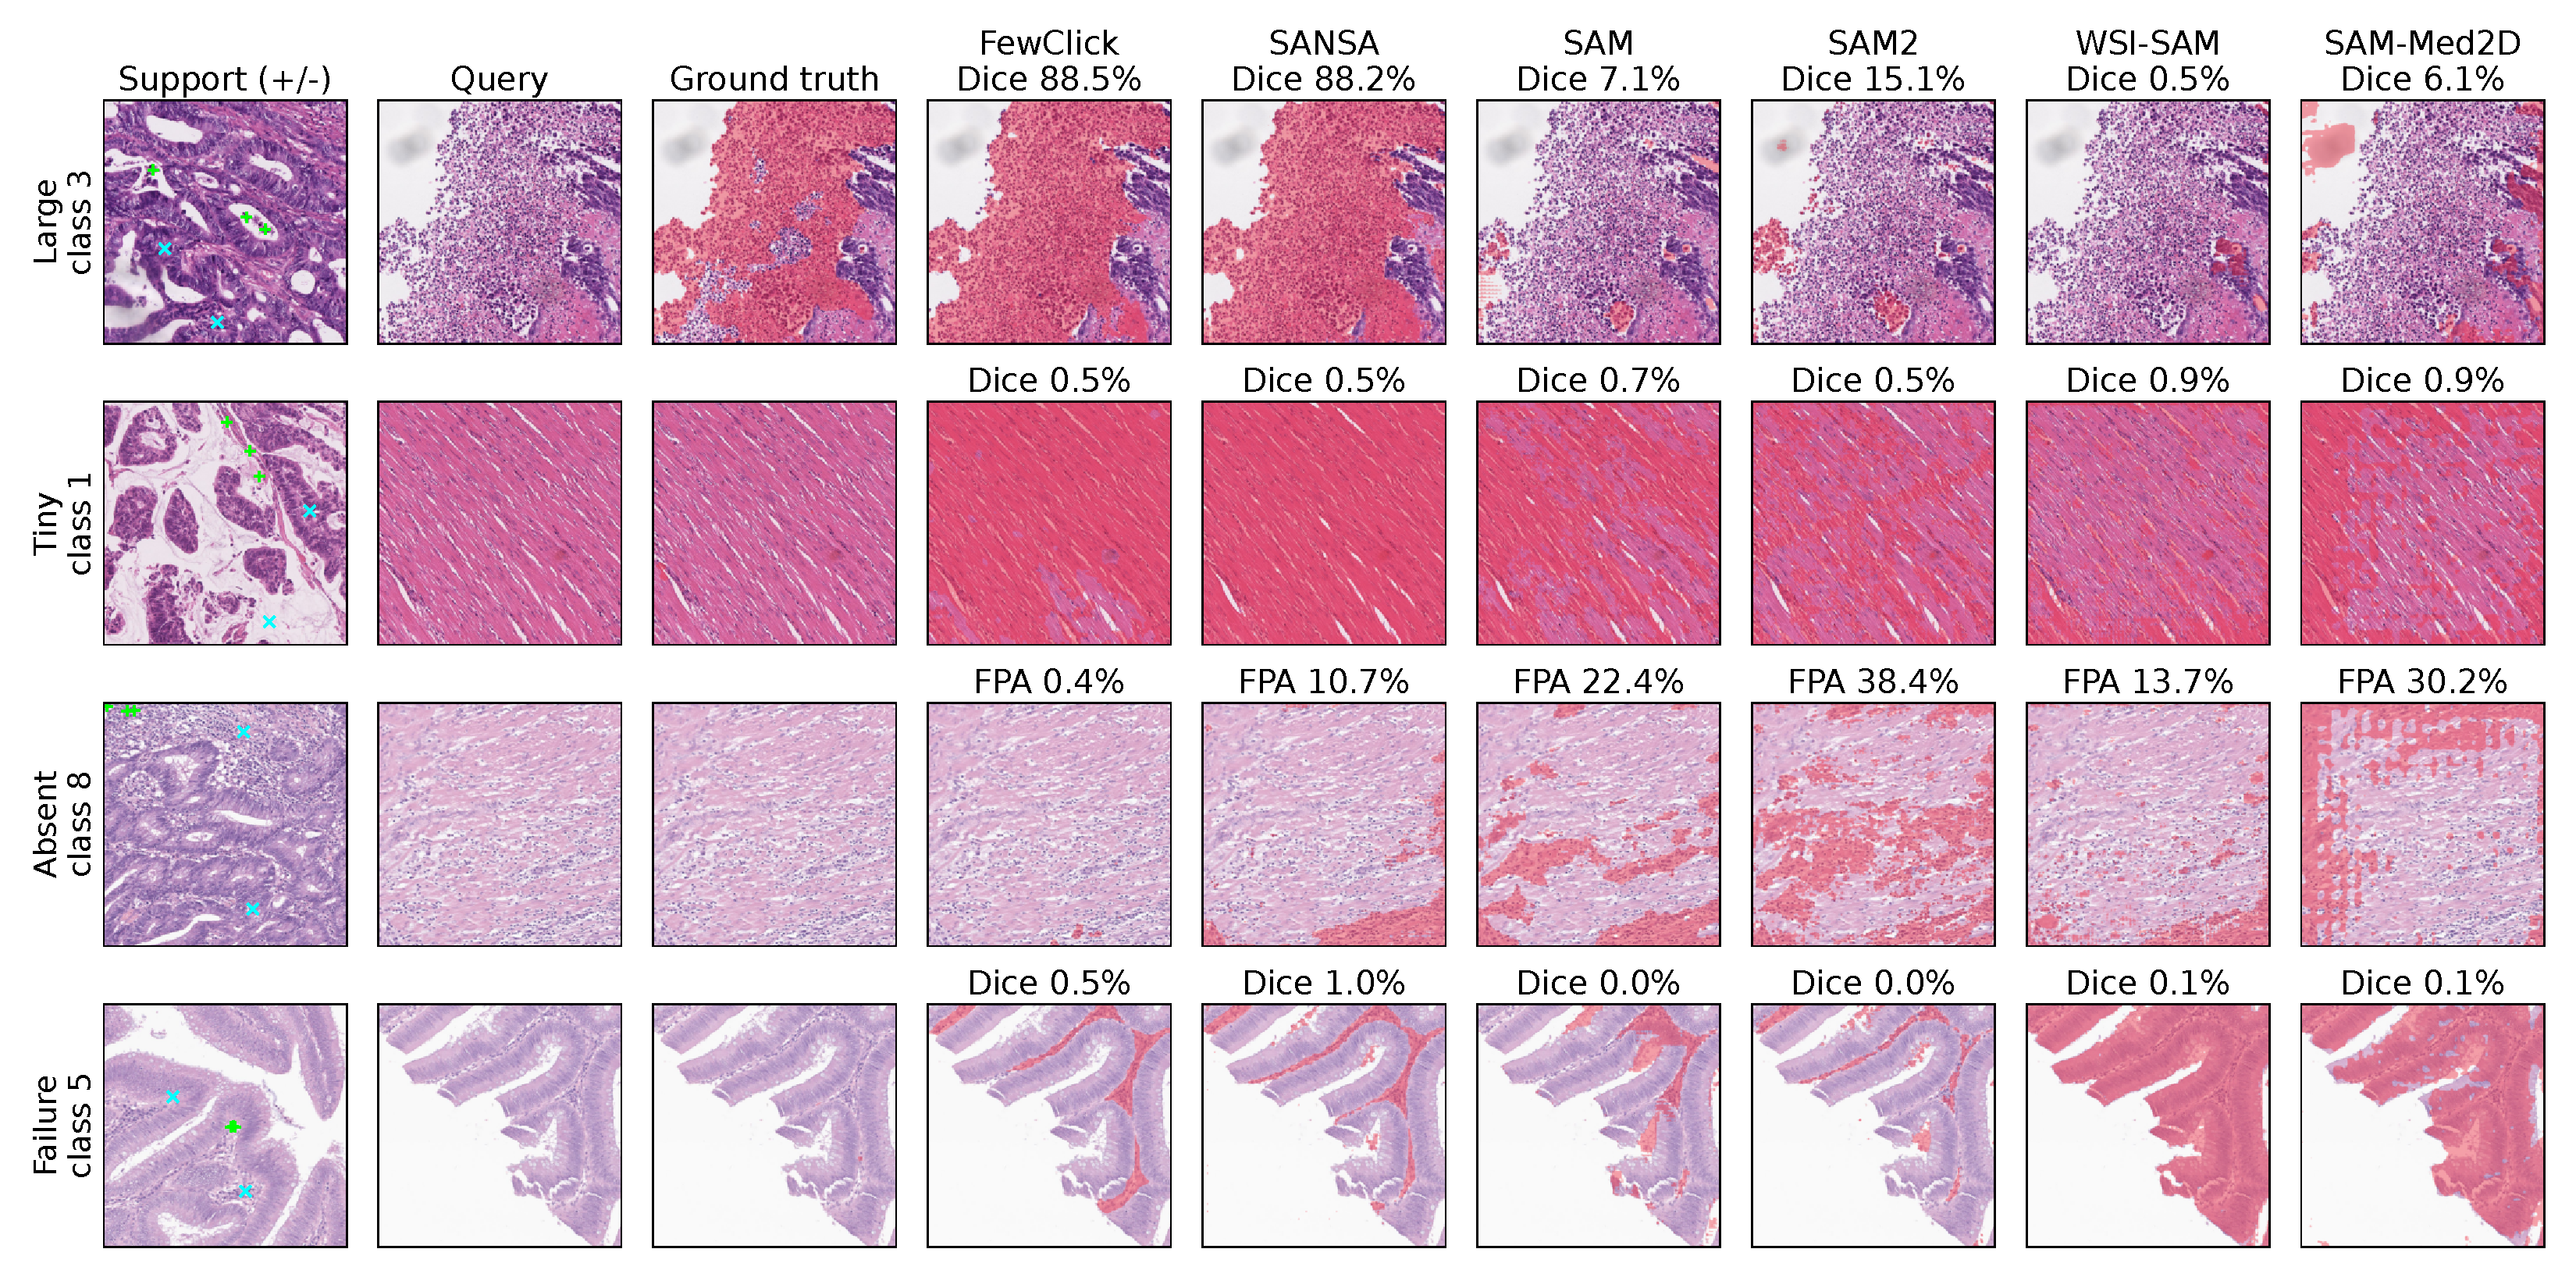
\includegraphics[width=\textwidth]{figures/figure3.pdf}
\caption{Remote qualitative cases: a large target, a tiny target, an absent target, and a low-Dice failure. Each row contains support clicks, query image, ground truth, and six-method predictions. Cases are chosen nearest to the group's FewClick median Dice (present) or FPA (absent), breaking ties by task index. Green plus and cyan cross markers denote positive and negative support clicks; red overlays denote target tissue. Panel scores are task-level Dice for present targets and FPA for the absent target. Metrics use the original $512\times512$ predictions.}
\label{fig:failures}
\end{figure*}

\subsection{Structural Ablations}
\begin{table}[t]
\centering
\caption{Matched structural ablations: (a) fine representation and dense transfer; (b) components of the fused model. P/L/S denote present-, large-, and small-target Dice; all values are percentages. Higher Dice and lower FPA are better.}
\label{tab:ablation}
\small
\setlength{\tabcolsep}{4pt}
\textbf{(a) Fine representation $\times$ dense transfer}\\[2pt]
\begin{tabular}{@{}llrrr@{}}
\toprule
Fine view & Transfer & P & L & FPA \\
\midrule
Whole & No & 39.19 & 73.81 & 6.71 \\
Whole & Yes & 39.97 & 76.51 & 8.10 \\
Tiled & No & 40.16 & 74.63 & 5.74 \\
Tiled & Yes & 40.87 & 76.84 & 7.04 \\
Fused & No & 40.92 & 75.37 & 5.61 \\
Fused & Yes & 42.11 & 78.49 & 7.75 \\
\bottomrule
\end{tabular}
\par\vspace{4pt}
\textbf{(b) Fused-model components}\\[2pt]
\begin{tabular}{@{}lrrrr@{}}
\toprule
Variant & P & L & S & FPA \\
\midrule
Full FewClick & 42.11 & 78.49 & 28.19 & 7.75 \\
No dense transfer & 40.92 & 75.37 & 28.04 & 5.61 \\
No region messages & 41.66 & 77.66 & 28.09 & 6.90 \\
\bottomrule
\end{tabular}
\end{table}

We train whole-patch, four-tile, and equal-fusion representations with and without dense transfer, forming a $2\times3$ comparison. Every model starts from the same public initialization, follows the $9{,}500$-task/$2{,}375$-update budget, and is evaluated on the same $11{,}000$ remote tasks.

\paragraph{Same-feature prototype baseline.}
Proto-MS predicts masks from positive and negative click prototypes and similarities using a lightweight convolutional decoder. It shares FewClick's frozen Phikon-v2, three physical views, equal whole/tiled fusion, seven encodings, and training budget. The shared subset contains 550 small-target, 262 large-target, and 275 absent tasks, sampled independently of predictions. Present Dice weights small/large strata by each tissue's original proportions. On these $1{,}087$ tasks, FewClick improves present Dice by 1.49 points (42.32 versus 40.83\%) and large-target Dice by 4.17 points (75.67 versus 71.50\%). Its absent-target FPA is higher, at 6.32\% versus 5.16\%. On the WSIs, fused whole-slide Dice rises from 42.13\% for Proto-MS to 45.65\% for FewClick. These overlap gains persist with identical pretrained features and input views.

\paragraph{Dense probability transfer.}
With fused features, adding dense transfer raises target-present Dice from 40.92\% to 42.11\% and large-target Dice from 75.37\% to 78.49\%; the recorded unrounded gains are 1.20 and 3.13 points. Small-target Dice increases from 28.04\% to 28.19\%. FPA rises from 5.61\% to 7.75\%, showing that this component primarily improves larger target regions while increasing target-absent responses.

\paragraph{Whole-patch and tiled representations.}
Fusion gives the highest present- and large-target Dice both with and without dense transfer (Table~\ref{tab:ablation}a), supporting the complementary use of complete architecture and local detail.

\paragraph{Cross-scale region messages.}
With the same views and seven backbone passes, replacing cross-scale region messages by identity mappings and removing cross-scale decoder edges gives 41.66\% present, 77.66\% large, and 28.09\% small Dice, with 6.90\% FPA. The 0.83-point large-target loss is smaller than the 3.13-point loss without dense transfer. Both components improve overlap while increasing absent FPA.

\paragraph{Learned versus fixed regions.}
With learned assignments replaced by a fixed spatial soft grid, matched retraining gives 42.04\% present Dice on the same $1{,}087$ tasks, compared with 42.32\% for FewClick. The 0.28-point gain from learned assignments is modest; the fixed grid gives slightly higher large-target Dice (76.02 versus 75.67\%), while learned regions reduce absent FPA from 6.67\% to 6.32\%.

\paragraph{Whole-slide component effects.}
On the WSIs, removing dense transfer reduces fused whole-slide Dice from 45.65\% to 41.70\%, while removing cross-scale region messages gives 44.27\%. Strict-remote Dice follows the same ordering: 43.04\% for FewClick, 39.42\% without dense transfer, and 41.89\% without region messages. The larger drop without dense transfer parallels its larger effect on large-target patch Dice.



\subsection{Efficiency and Prompt Sensitivity}
\begin{table}[t]
\centering
\caption{Mean latency and cache size over 100 tasks on one RTX 5880 Ada GPU. First prediction includes reading and encoding; changed-prompt prediction reuses image features. Cache size includes one support--query feature pair and prompt memory.}
\label{tab:efficiency}
\small
\setlength{\tabcolsep}{4pt}
\begin{tabular}{@{}lrrr@{}}
\toprule
Method & First (ms) & Changed (ms) & Cache (MiB) \\
\midrule
FewClick & 1539.2 & 43.0 & 16.39 \\
SANSA & 1226.3 & 39.1 & 212.38 \\
SAM & 1191.8 & 18.0 & 16.00 \\
SAM2 & 1297.9 & 16.3 & 40.00 \\
WSI-SAM & 767.9 & 36.3 & 34.00 \\
SAM-Med2D & 863.9 & 17.7 & 1.00 \\
\bottomrule
\end{tabular}
\end{table}

Six methods are timed sequentially on one GPU over 100 tasks after three warm-ups. First prediction includes reading and encoding with three positive/two negative clicks; changed-prompt prediction reuses features with one positive/one negative. GPU-synchronized timings exclude loading and scoring.

FewClick averages 1539.2\,ms initially and 43.0\,ms after a prompt change, versus SANSA's 1226.3/39.1\,ms, with a 16.39 versus 212.38\,MiB cache (Table~\ref{tab:efficiency}). FewClick thus uses 92.3\% less cache while retaining a 43.0\,ms prompt-update time. Shared-GPU whole-slide processing averages 98.0 minutes per slide for all FewClick targets, including query reading/encoding, decoding, fusion, scoring, and saved-mask verification.

On 330 tasks selected by tissue/size-stratified hashing (220 present and 110 absent), reducing prompts from three positive/two negative to one positive/one negative lowers FewClick/SANSA Dice from 53.18/52.83\% to 51.14/51.03\%. With three positives, a second negative reduces FewClick FPA from 9.80\% to 8.20\%. Two- or five-pixel radial perturbations in the $512\times512$ support grid change Dice by at most 0.31 points.

\subsection{Target Size, Boundaries, and Failure Analysis}

On $5{,}204$ small-target tasks, FewClick achieves 28.19\% macro Dice versus SANSA's 27.65\%. Both remain below 8\% Dice for targets occupying less than 1\% of valid area (7.68/7.59\%). For the $1$--$5\%$ and $5$--$20\%$ strata, FewClick/SANSA Dice rises to 36.98/35.59\% and 59.43/59.05\%, respectively.

FewClick's overall precision is 39.67\%, above SANSA's 38.21\%, whereas recall is 67.90\% versus 77.75\% and boundary F1 is 25.86\% versus 29.25\%. On large targets, FewClick improves both precision (77.69\% versus 76.65\%) and recall (83.66\% versus 82.98\%), while boundary F1 is lower (40.35\% versus 45.51\%). Its stronger large-region coverage thus coexists with less accurate fine contours.

Figure~\ref{fig:failures} shows large, tiny, absent, and low-Dice cases. In the absent-target example, FewClick/SANSA FPA is 0.40/10.67\%. At 0.24\% target area, FewClick obtains 0.51\% Dice with extensive non-target responses.
